% This is LLNCS.DEM the demonstration file of
% the LaTeX macro package from Springer-Verlag
% for Lecture Notes in Computer Science,
% version 2.3 for LaTeX2e
%
\documentclass{llncs}
%
\usepackage{makeidx} % allows for indexgeneration
\usepackage{graphicx}
\usepackage{multicol}
\usepackage{subfigure}
\usepackage{mathptmx} % use Times fonts if available on your TeX system
\usepackage{setspace}
%
\begin{document}
\title{Robotic Validation of an Inter-disciplinary Generic\\
Model of Self-regulated Division of Labour\\ in Social Systems
\thanks{This research has been funded by the Engineering and Physical Sciences Research Council (EPSRC), UK, grant reference EP/E061915/1.}
}
%\subtitle{Do you have a subtitle?\\ If so, write it here}
\titlerunning{Robotic Validation of an Inter-disciplinary Generic Model\\
 of Self-regulated Division of Labour in Social Systems } % if too long for running head
\author{Md Omar Faruque Sarker \and
Torbjorn Dahl %etc.
}
%\authorrunning{Short form of author list} % if too long for running head
\institute{
Robotic Intelligence Lab,
Newport Business School\\
University of Wales, Newport,
Allt-yr-yn Campus\\ Allt-yr-yn Avenue, Newport, NP205XR, UK\\
\email{Mdomarfaruque.Sarker@newport.ac.uk\\
Torbjorn.Dahl@newport.ac.uk}
}
%\date{Received: / / Accepted: / / }
% The correct dates will be entered by the editor
\maketitle
\begin{abstract}
Multi-agent task allocation or division of labour (DoL) is a challenging research issue in the field of multi-agent and multi-robot systems. In order to address this issue, existing approaches such as, predefined (off-line) and emergent (real-time) task-allocation, fail to scale well with large number of robots. Typically, increased communication interference and decreased bandwidth among agents are major causes of this problem. Unlike the swarm robotic approach, which is inspired by biological systems alone and commonly aims for minimal intelligence agents, we propose to solve DoL in multi-robots based on a set of observed generic rules of DoL from biological and human social systems. These bottom-up rules describe the phenomena of self-regulated DoL in terms of attractive fields between robots and tasks. The concrete form of these rules, termed as \textit{attractive filed model} (AFM), offers a scalable solution to the above DoL problem. Unlike having strong dependence to communication mediums by most of the existing approaches, our model states that self-regulatory DoL can be established by AFM without maintaining a strong form of on-line communication. Our approach has been validated by experiments with 16 physical E-puck robots in an area of about 4$m^2$.
%\keywords{First keyword \and Second keyword \and More}
%% \PACS{PACS code1 \and PACS code2 \and more}
%% \subclass{MSC code1 \and MSC code2 \and more}
\end{abstract}
%\addtolength{\parskip}{-3.5mm}
\section{Introduction}
\label{sec:intro}
%\vspace{2mm}
Multi-agent task allocation or division of labour (DoL) is a challenging research issue in the field of multi-agent and multi-robot systems e.g., swarm robotics \cite{Swarm}. In order to address this issue, existing approaches e.g., predefined (off-line) and emergent (real-time) task-allocation, fail to scale well with large number of agents. Typically, increased communication interference and decreased bandwidth among agents are major causes of this problem. Unlike the swarm robotic approach, which is inspired by biological systems alone and commonly aims for minimal intelligence agents, we propose to solve DoL in multi-agents based on a set of observed generic rules of DoL from biological and human social systems. These bottom-up rules describe the phenomena of self-regulated DoL in terms of attractive fields between agents and tasks. The concrete form of these rules, termed as \textit{attractive filed model} (AFM) \cite{Elsa}, offers a scalable solution to the above DoL problem. Unlike having strong dependence to communication mediums by most of the existing approaches, our model states that self-regulatory DoL can be established by AFM without maintaining a strong form of on-line communication.
%\vspace{4mm}
We have investigated the performance of two different communication strategies for self-regulated DoL among a larger robot teams: centralized and local. These forms of communications typically resemble to message broadcast and peer-to-peer (P2P) communications respectively.

Section 2 describes our model of self-regulated DoL and an associated model of communication for different entities of our system. Section 3 introduces our experiment set-up and interaction of hardware and software modules. Section 4 presents our experiment design with parameters and observables. Section 5 discusses our experimental results.  Section 6 concludes this paper. 
%
%%%%%%%%%%%%%%%%%%%%%%%%%%%%%%%%%%%%%%%%%%%%%%%%%%%%%%%%%%%%%%%%%%%%%%%%%%%%%%%%%%%%
%\addtolength{\topskip}{-15mm}
\section{Modeling}
\label{sec:model}
\subsection{Model for Self-Regulatory DoL}
Our model of self-regulated DoL is based on AFM. It provides us a generic framework for implementing self-regulatory DoL in robots. Here we briefly describe how this model gives our robots self-regulatory DoL behaviours, particularly task-specialization, concurrency, flexibility and robustness.
%%
\begin{figure}
\begin{minipage}[t]{0.48\linewidth}
\centering
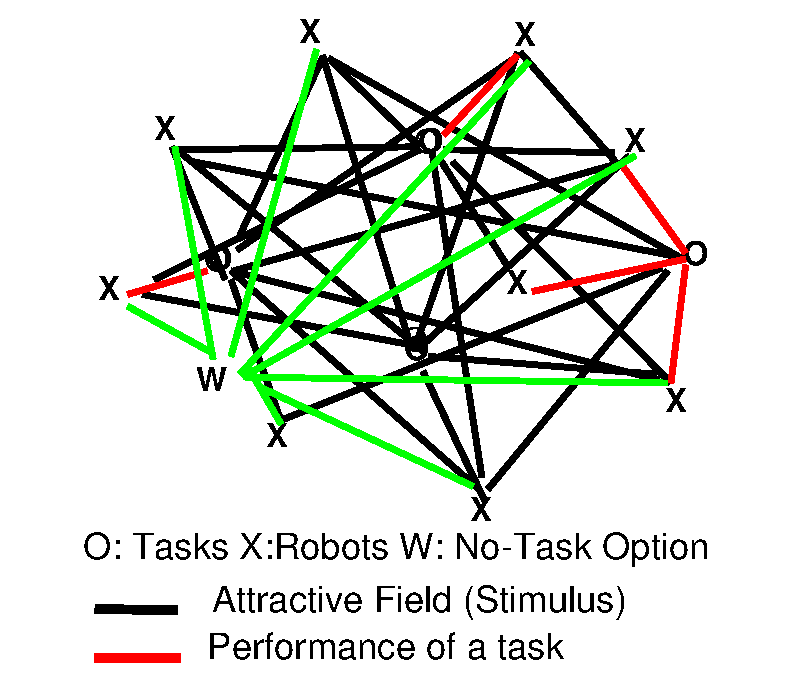
\includegraphics[height=5cm, angle=0]
{../dia-files/AFM-Diag2.eps}
 %figure caption is below the figure
\caption{\small Atrractive Filed Model}
\label{fig:afm} % Give a unique label
\end{minipage}
\hspace{0.5cm}
\begin{minipage}[t]{0.48\linewidth}
\centering
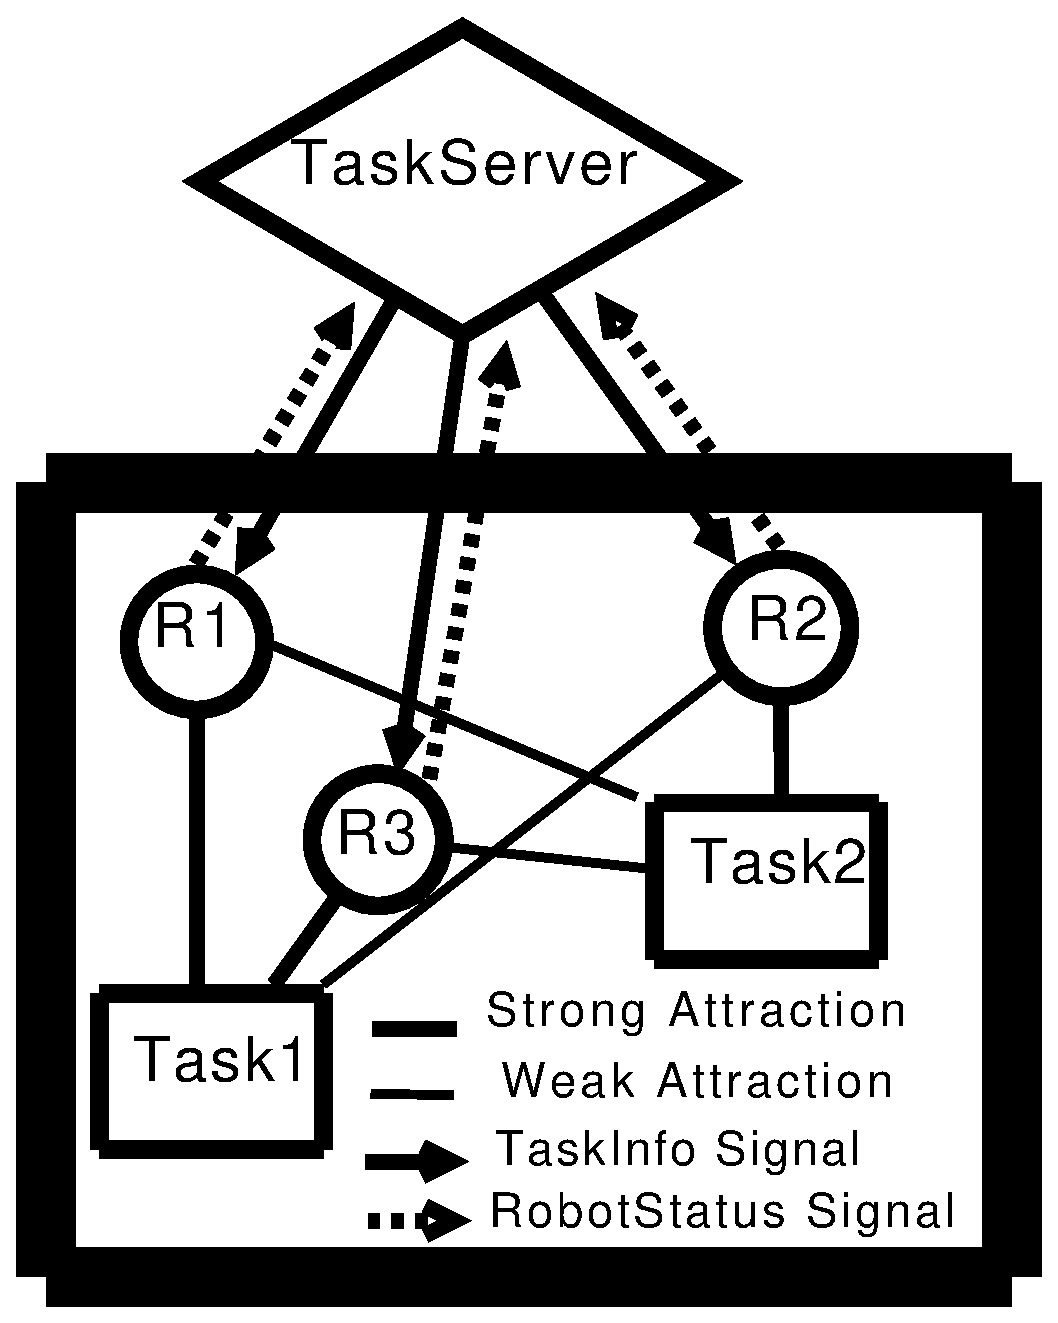
\includegraphics[height=5cm, angle=0]{../dia-files/CentralizedComm.eps}
\caption{\small Centralized Communication Model}
\label{fig:ccm} % Give a unique label
\end{minipage}
\end{figure}
%%
Let us consider a manufacturing shop floor scenario where N number of mobile robots are required to attend to M number of shop tasks spread over a fixed area A. Let these tasks be represented by a set of small rectangular boxes resembling to manufacturing machines. Let $R_1$, $R_2$ … $R_n$ be the set of all robots and $J_1$, $J_2$ … $J_m$ be the set of all tasks. Each task $j$ has an associated task-urgency $\phi_j$ that indicates its relative importance over time. If a robot attends to a task $j$ in x$^{th}$ time-step, value of $\phi_j$ will decreases by a small amount $\delta_\phi$ in (x+1)$^{th}$ time-step. On the other hand, if a task has not been served by any robot in x$^{th}$ time-step, $\phi_j$ will increase by another small amount in (x+1)$^{th}$ time-step. In order to complete a shop task $J_1$, a robot $R_1$ needs to reach within a fixed boundary $D_j1$ of $J_1$. If a robot completes a task $j$ we say that it learns about it and this will increase robot's likelihood of selecting that task in next step. We call this variable affinity of a robot to that task as its sensitization $k_j$ . If a robot does not do a task $j$ for some time, we say that it forgets about $j$ and $k_j$ has been decreased.\\
According AFM, all robots will establish attractive fields to all tasks due to the presence of a system-wide continuous flow of information. The strength of these attractive fields called stimulus will vary according to the distances between robots and tasks, task-urgencies and corresponding sensitizations of robots. This is encoded in Eq. \ref{eqn1}.
%\addtolength{\abovedisplayskip}{-15mm}
\begin{small}
\begin{multicols}{2}
\begin{equation}
S_{j}^{i} = tanh\{\frac{k_{j}^{i}}{d+\delta } \phi _{j}\}
\label{eqn1}
\end{equation}
\vspace*{0.25cm}
\begin{equation}
P_{j}^{i} = \frac{S_{j}^{i}}{\sum_{j}^{}S_{j}^{i}}
\label{eqn2}
\end{equation}
\end{multicols}
\end{small}
%\addtolength{\belowdisplayskip}{-1mm}
%\vspace{2mm}
Eqn \ref{eqn1} says that the stimuli of a robot $i$ to a particular task $j$, $(S_{j}^{i})$ depends on robot's spatial distance $d$ to $j$, level of sensitization to that task ($k_{j}^{i}$) and perceived urgency of that task ($\phi _{j}$). We use a vary small value $\delta$ in \ref{eqn1} to prevent division by zero. The probability of selecting each task has been determined by a probabilistic method outlined in Eq. \ref{eqn2} .
AFM suggests concurrency of a self-regulatory system by specifying at least two task options: 1) doing a task and 2) doing no task. In robots, the latter can be be treated as random walking. So in any time-step a robot will choose from M+1 tasks. Let $T_a$ be the allocated time to accomplish a task. If $R_1$ can enter inside the task boundary within $T_a$ time it waits there until $T_a$ elapsed. Otherwise it will select a different task.
 
\subsection{Model for Communication}
In order to establish a system-wide continuous flow of information, one needs to implement a suitable communication system. Here we have presented two models of communication for our above manufacturing shop-floor scenario.
%% 
As shown in Fig. \ref{fig:ccm}, in this model there exists a centralized Task-Server that is responsible for disseminating task information to robots. The content of task information can be location of task in the environment, urgency and so on. Task server delivers this information by emitting TaskInfo signals periodically. The method of signal emission depends on a particular communication technology. For example, in a wireless network it can be a message broadcast.
Task-Server has another interface for catching feedback signals from robots. This RobotStatus signal may contain what task a robot is currently doing, its device status and so on. Task-Server uses this information to update task information such as, task-urgency. This up-to-date information is sent in TaskInfo signal.
In Fig. \ref{fig:ccm} an initial configuration of this model has been presented. Upon receiving an initial TaskInfo signal robot $R_1$ and $R_2$ shows strong attractions towards $Task1$ and robot $R_3$ shows strong attraction toward $Task2$. This can be inferred from Eq. \ref{eqn1}. If the initial task urgencies and sensitizations are same for all tasks, a robot will be strongly attracted towards a task that is relatively closer to it.
%%%%%%%%%%%%%%%%%%%%%%%%%%%%%%%%%%%%%%%%%%%%%%%%%%%%%%%%%%%%%%%%%%%%%%%%%%%%%%%%%%% 
\section{Implementation}
\label{sec:impl}
\begin{figure}
\centering
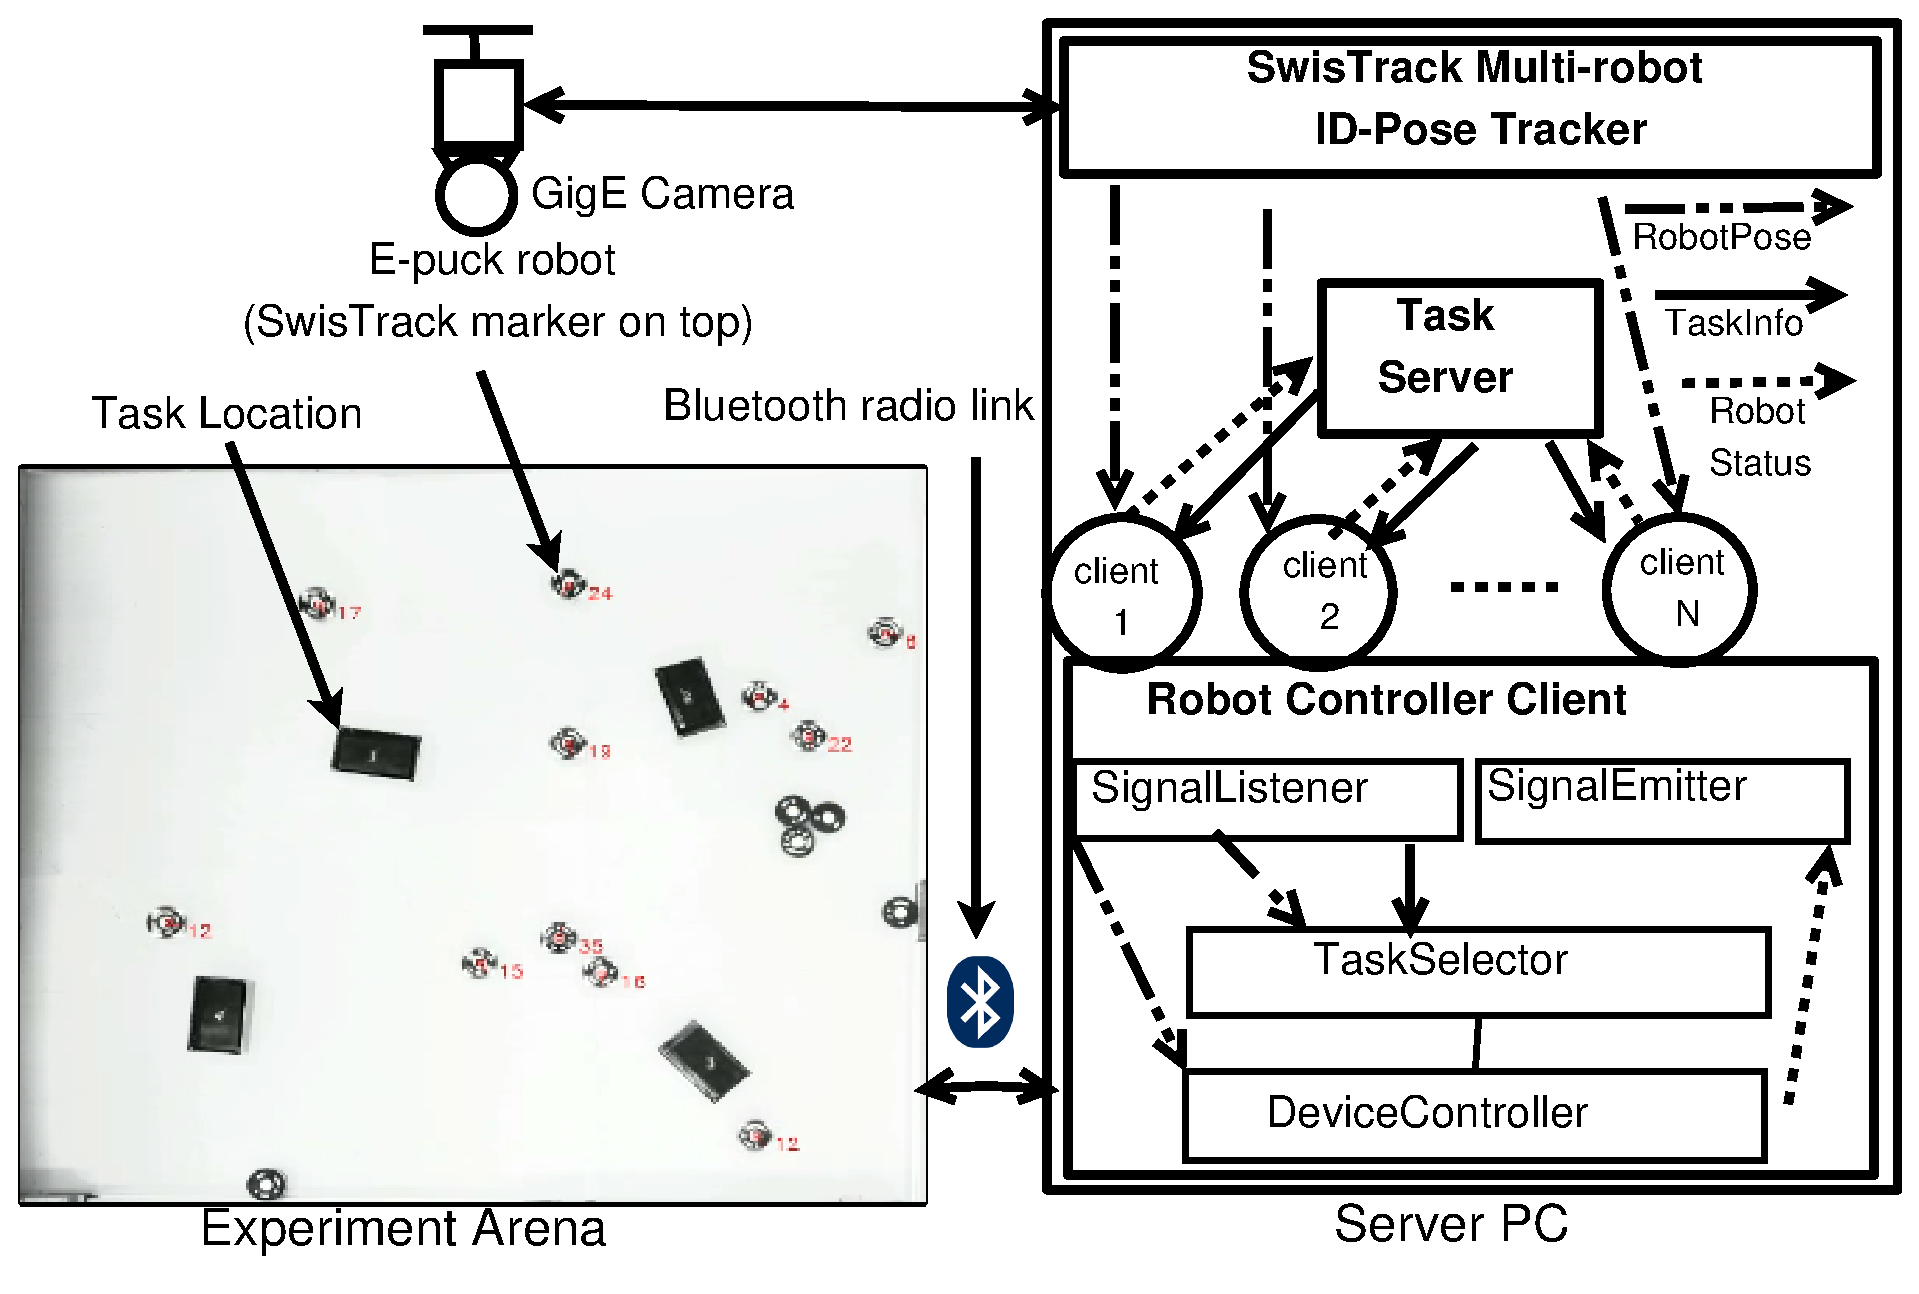
\includegraphics[height=7cm, angle=0]
{../dia-files/RIL-Expt-Setup1.eps}
 %figure caption is below the figure
\caption{\small Hardware and software setup}
\label{fig:setup} % Give a unique label
\end{figure}
 
We have developed a system where up to 40 E-puck robots \cite{Epuck} can operate together according to the generic rules of the AFM.  In order to track the robots we use SwisTrack \cite{SwisTrack}, a state of the art open-source, multi-agent tracking system, along with an overhead 16-megapixel GigE camera. This set-up gives us the position, heading and id of each of the robots at a frequency of 1. The interaction of the hardware and software of our system is illustrated in Fig. \ref{fig:setup}. 

For inter-process communication (IPC), we have used D-Bus technology \cite{DBus}. We have developed a IPC  component for SwisTrack (hereafter called as SwisTrack D-Bus Server) that can broadcast id and pose of all robots in real-time over D-Bus.

Apart from SwisTrack, we have implemented two major software modules: Task-Server and Robot-Controller-Client (RCC). They are developed in Python with state-of-art Multiprocessing module \cite{Multiprocessing}. This python module simplifies our need to manage data sharing among different sub-processes.  As shown in Fig. \ref{fig:setup}, RCC consists of four sub-processes: SignalListener, SignalEmitter, TaskSelector, DeviceController. SignalListener  catches RobotPose and TaskInfo signals from SwisTrack D-Bus Server and Task-Server respectively. SignalEmitter emits RobotStatus signal for TaskServer. TaskSelector selects a particular task based on information obtained from TaskInfo and RobotPose signals. This selected task has been notified to DeviceController that actually moves the robot to a target task.   DeviceController uses Bluetooth radio link as a communication medium between RCC and physical E-puck. Data sharing and synchronization among all four sub-processes are done using Data-manger and Event interfaces of Python Multiprocessing module. Similar to RCC, Task-Server also has three sub-processes: SignalListener, SignalEmitter and TaskInfoUpdater. SignalListener  listens RobotInfo signal and passes corresponding info to TaskInfoUpdater that updates task urgency of all tasks based on AFM rules. The updated information is then encoded as TaskInfo signal and emitted by SignalEmitter. TaskInfo signal also contains location of all tasks that we have provided to TaskServer as start-up arguments. 

To recap, our system works by repeating the following steps:

\begin{itemize}
\item SwisTrack grabs overhead camera image and finds id and pose of all robots.  SwisTrack D-Bus Server periodically  broadcast them as RobotPose D-Bus signal.
\item All RCC catch their individual RobotPose signal and a common TaskInfo signal from SwisTrack D-Bus Server and TaskServer respectively. They select a particular task or random walk based on AFM. If a physical link between an E-puck robot and a RCC is established, this selected task is then started to execute. When a task-execution starts each RCC emits its status signal over D-Bus.
\item TaskServer updates task-urgencies after processing RobotStatus signal received from robots. This updated task-urgencies are then encoded in TaskInfo signal and emitted by TaskServer in next step.
\end{itemize}
%%%%%%%%%%%%%%%%%%%%%%%%%%%%%%%%%%%%%%%%%%%%%%%%%%%%%%%%%%%%%%%%%%%%%%%%%%%%
\section{Experiment Design}
\label{sec:expt-design}
In order to validate AFM in robots we have designed a set of centralized communication experiments as outlined in \ref{sec:impl}. Here we describe our experimental 
 and observables.
%
\begin{table}
\caption{Experimental parameters}
\label{table:params}
\begin{center}
\begin{tabular}{|l||c|}
\hline Parameter & Value\\
\hline Total number of robots ($N$) & 16\\
\hline Total number of tasks ($M$) & 4\\
\hline Experiment area ($A$) & 4 $m^2$\\
\hline Intial task urgency ($\Phi_{INIT}$) & 0.5\\
\hline Task urgency increase rate ($\Delta\phi_{INC}$) & 0.005\\
\hline Task urgency decrease rate ($\Delta\phi_{DEC}$) & 0.0025\\
\hline Intial sensitization ($K_{INIT}$) & 0.1\\
\hline Sensitization increase rate ($\Delta k_{INC}$) & 0.03\\
\hline Sensitization decrease rate ($\Delta k_{DEC}$) & 0.01\\
\hline A very small distance ($\delta$)& 0.000001\\
\hline Task info update interval ($\Delta TS_{u}$) & 5s\\
\hline Task info signal emission interval ($ \Delta TS_{e}$)& 2.5s\\
\hline Robot's task time-out interval ($\Delta RT_{to} $)& 10s\\
\hline
\end{tabular}
\end{center}
\end{table}
% 
\subsection{Parameters}
Table \ref{table:params} lists a set of essential parameters of our experiments. The following relationships are maintained for selecting task-urgency and sensitization parameters.
\begin{small}
\begin{equation}
\Delta\phi_{DEC} = \Delta\phi_{INC} \times \frac{N}{2 \times M}
\label{eqn:task-urgency}
\end{equation}
%
\begin{equation}
\Delta k_{DEC} = \frac{\Delta k_{INC}} {M - 1} 
\label{eqn:sensitization}
\end{equation}
\end{small}
%
\subsection{Observables}
\textbf{Changes in task-urgency ($\Delta \Phi$): }
In our experiments,  urgency of each task in each step will be logged. From the above design of task urgency, we can see that if a task is not served by any robot for 100 consecutive steps in 500s  urgency of that task will reach from 0.5 to its maximum urgency  1.0. On the other hand, if a task is served by only one robot for 200 consecutive steps in 1000s urgency of that task will be 0. But in real experiment it is more likely that more than one robot will serve a task. So urgency of a task will  decrease $\Delta\phi_{DEC}$ times number of working robots on that task \cite{Elsa}. The overall changes in task urgencies will show the convergence behaviour of our system. A stable convergence will most likely map to a stable division of labour of the system.\\
%
\textbf{Changes in sensitization ($\Delta K$): }
According AFM, as robots will do tasks they will specialize on each task by increasing or decreasing sensitizations (learning and forgetting).  From our above design, we can see that if a robot starts doing a task with an initial sensitization of 0.1 and it repeatedly does it for 30 consecutive steps, we will be able to say that it has learnt it completely. On the other hand,  with an initial sensitization of 0.1 if a robot does not do a task for 10 consecutive steps we will be able to say that it has forgotten that task completely.\\
%
\textbf{Changes in robot motion ($\Delta Tr$): }
As we might guess that initially the task urgencies will be relatively higher for all tasks so robots will need to do a lot of movements by switching from one tasks to another. But as the system convergences overall robot motions will be decreased. In order to observe this phenomenon we log the pose of robots in each time they receive pose signals.\\
%
\textbf{D-Bus Signals emitted by Task server ($S_f$):} 
In order to measure the communication load on our system and to benchmark Task server's D-Bus signalling performance we are also interested to log its D-Bus signals. Since the emission of signals happens in fixed time interval it is more likely that the overall communication load on the system will remain constant over time.
%
%%%%%%%%%%%%%%%%%%%%%%%%%%%%%%%%%%%%%%%%%%%%%%%%%%%%%%%%%%%
% 
\section{Results and Discussions}
\label{sec:results}
%
\begin{figure}
\begin{minipage}[t]{0.5\linewidth}
\centering
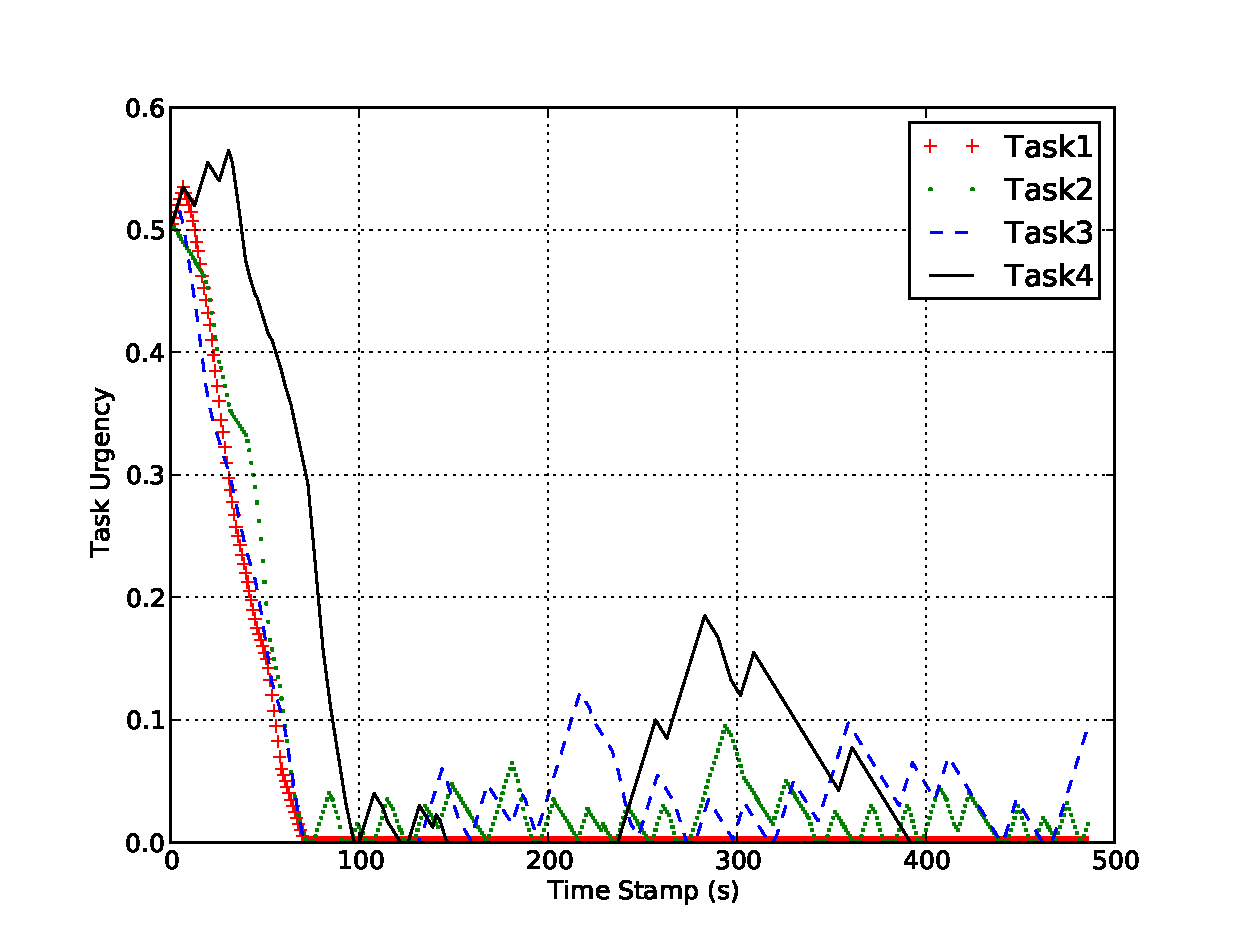
\includegraphics[height=5cm, angle=0]
{images/global/GlobalPlotUrgencyLog-2010Feb18-151600-clear.eps}
 %figure caption is below the figure
\caption{\small Task urgency changes in centralized communication experiments}
\label{fig:raw-urgencies} % Give a unique label
\end{minipage}
\hspace{0.5cm}
\begin{minipage}[t]{0.5\linewidth}
\centering
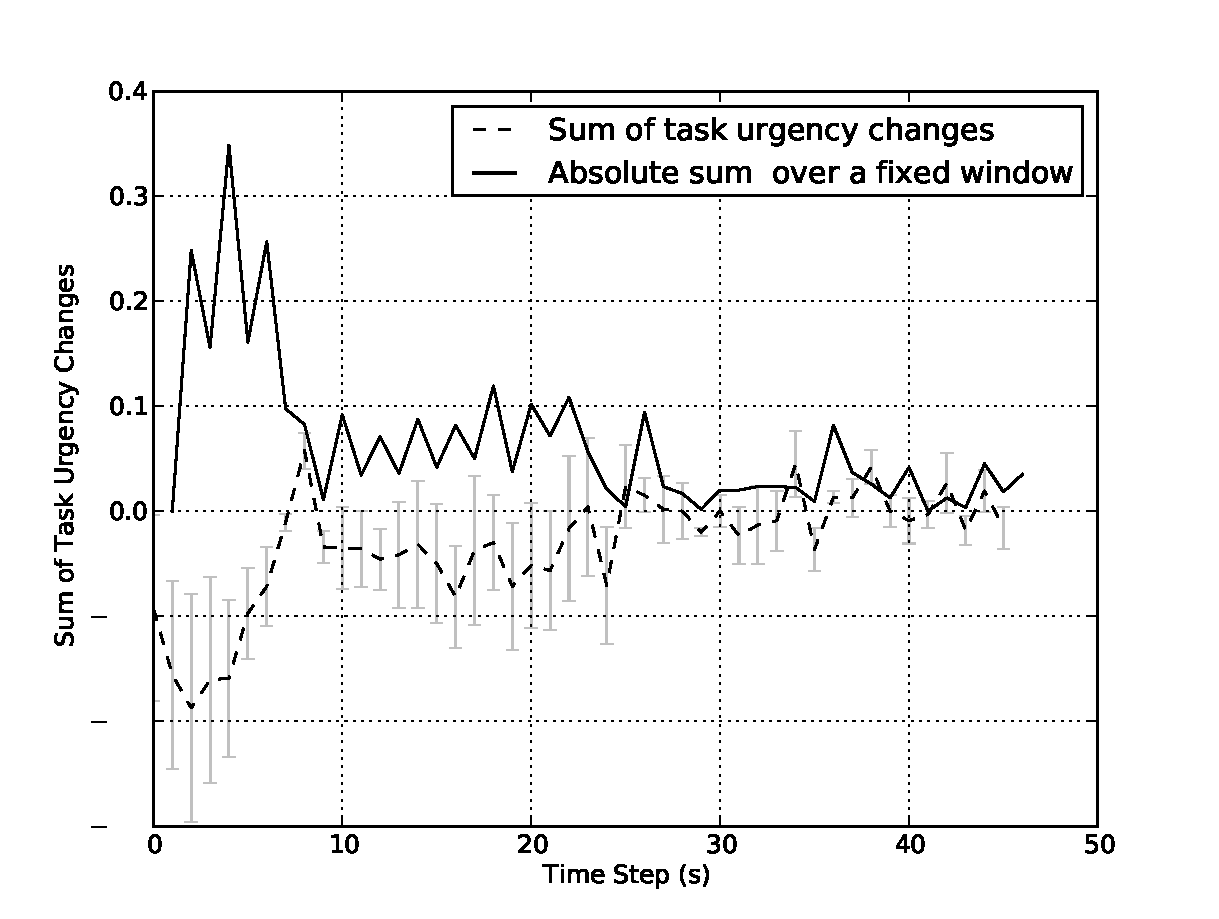
\includegraphics[height=5cm, angle=0]{images/global/TaskUrgencyConvergence-step2-th-p1.eps}
\caption{\small Task urgency convergence in centralized communication experiments}
\label{fig:urgency-convergence} % Give a unique label
\end{minipage}
\end{figure}
%%
%%% Sensitization and Translation %%%
\begin{figure}
\begin{minipage}[t]{0.5\linewidth}
\centering
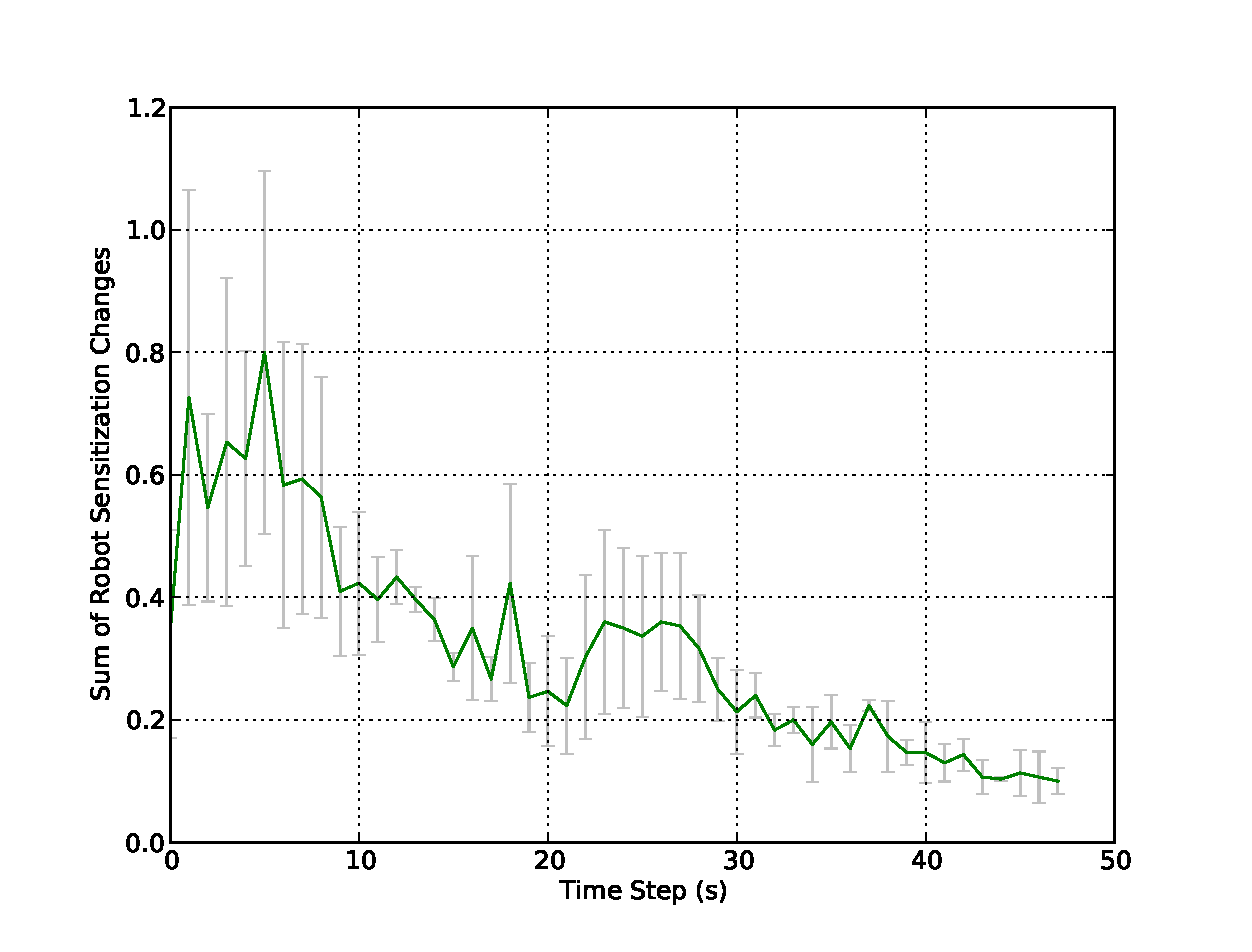
\includegraphics[height=5cm, angle=0]
{images/global/RobotSensitizationStat-Total-50steps.eps}
 %figure caption is below the figure
\caption{\small Sensitization changes in centralized communication experiments}
\label{fig:sensitization-stat} % Give a unique label
\end{minipage}
\hspace{0.5cm}
\begin{minipage}[t]{0.5\linewidth}
\centering
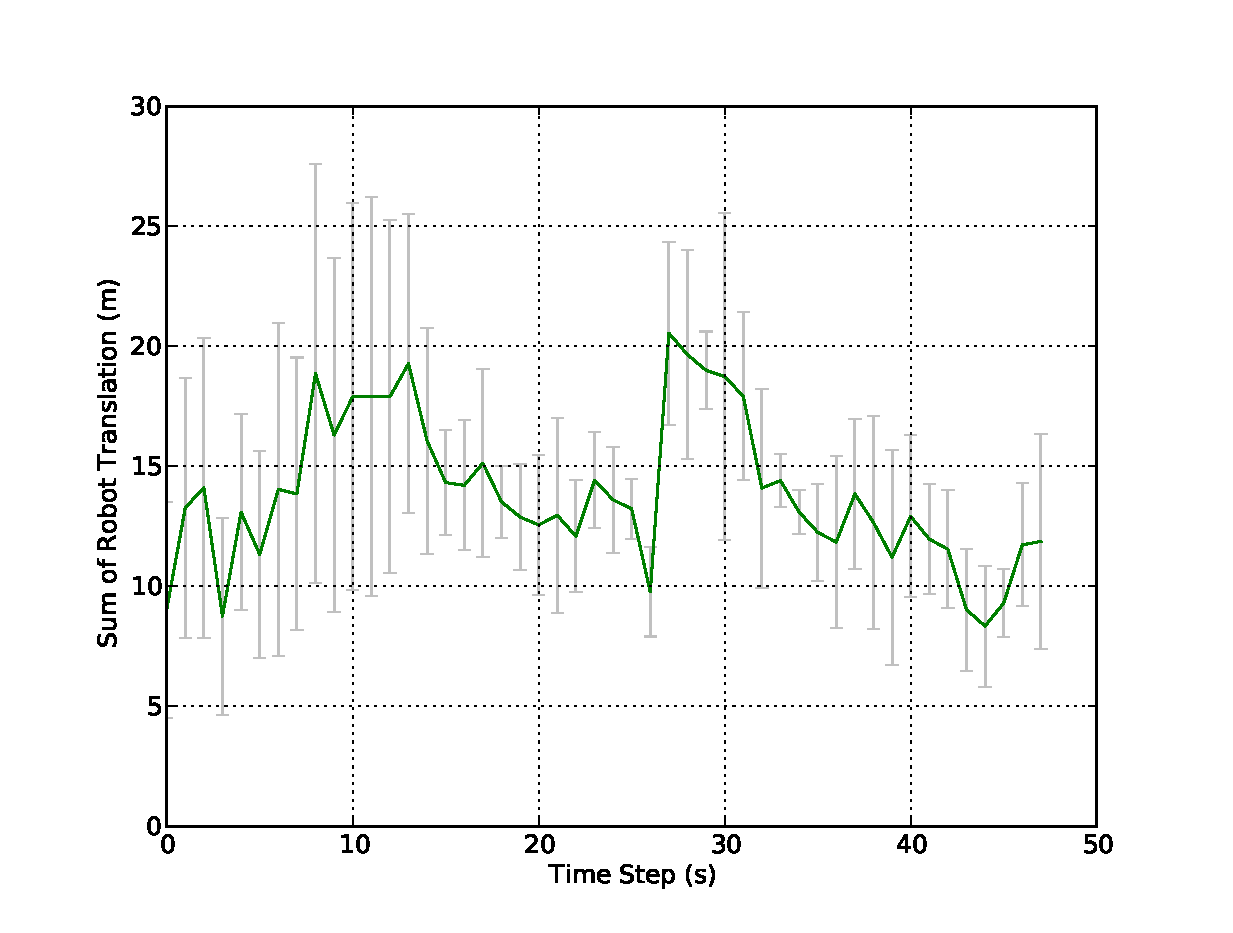
\includegraphics[height=5cm, angle=0]{images/global/DeltaTranslationStat.eps}
\caption{\small Sum of robot translation in centralized communication experiments}
\label{fig:translation-stat} % Give a unique label
\end{minipage}
\end{figure}
%%
%%% Communication load %%%
\begin{figure}
\begin{minipage}[t]{0.5\linewidth}
\centering
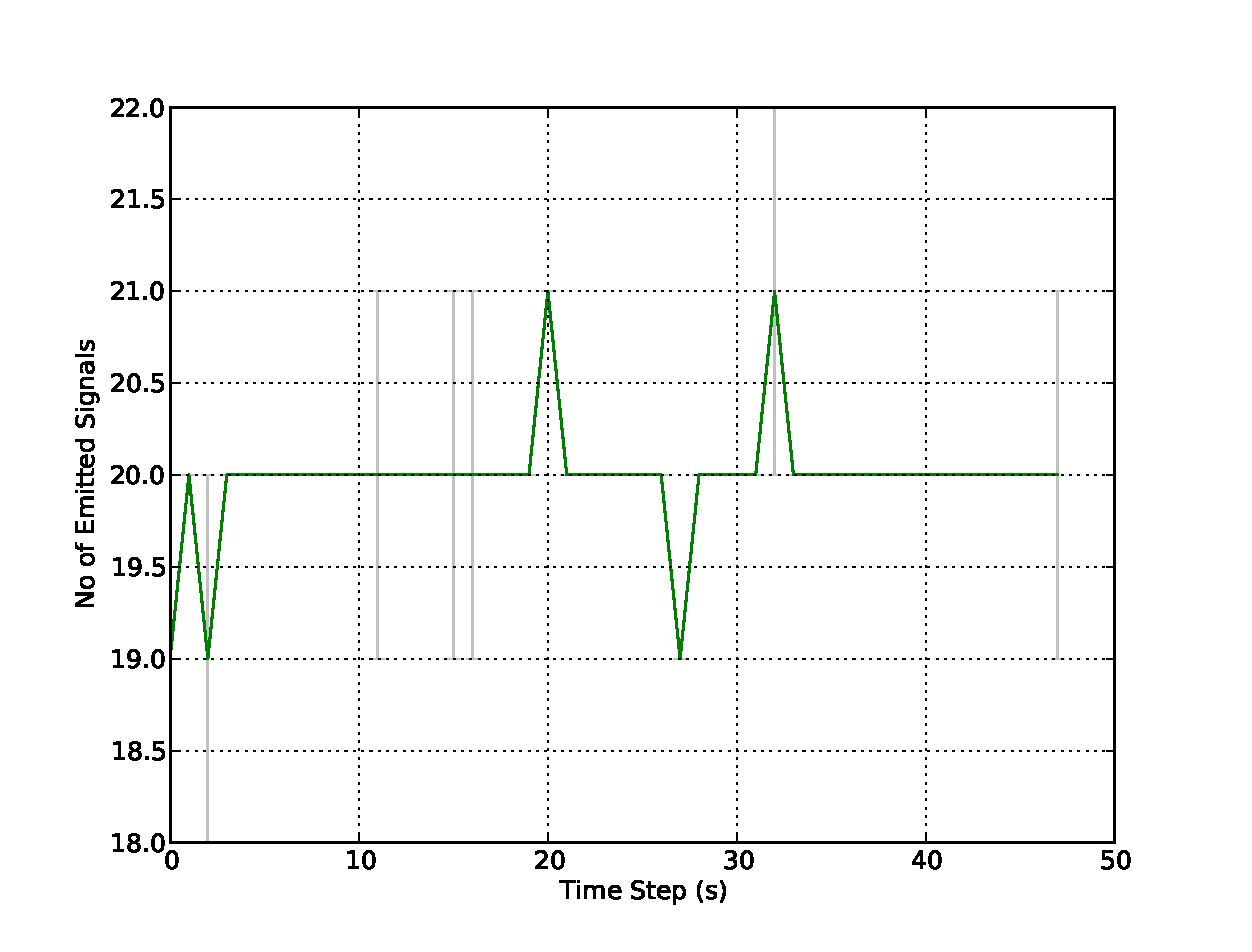
\includegraphics[height=5cm, angle=0]
{images/global/Global-SignalingFreqStat.eps}
 %figure caption is below the figure
\caption{\small Task server's frequency of signalling in centralized communication experiments}
\label{fig:signal-frequency-stat} % Give a unique label
\end{minipage}
\hspace{0.5cm}
\begin{minipage}[t]{0.5\linewidth}
\centering
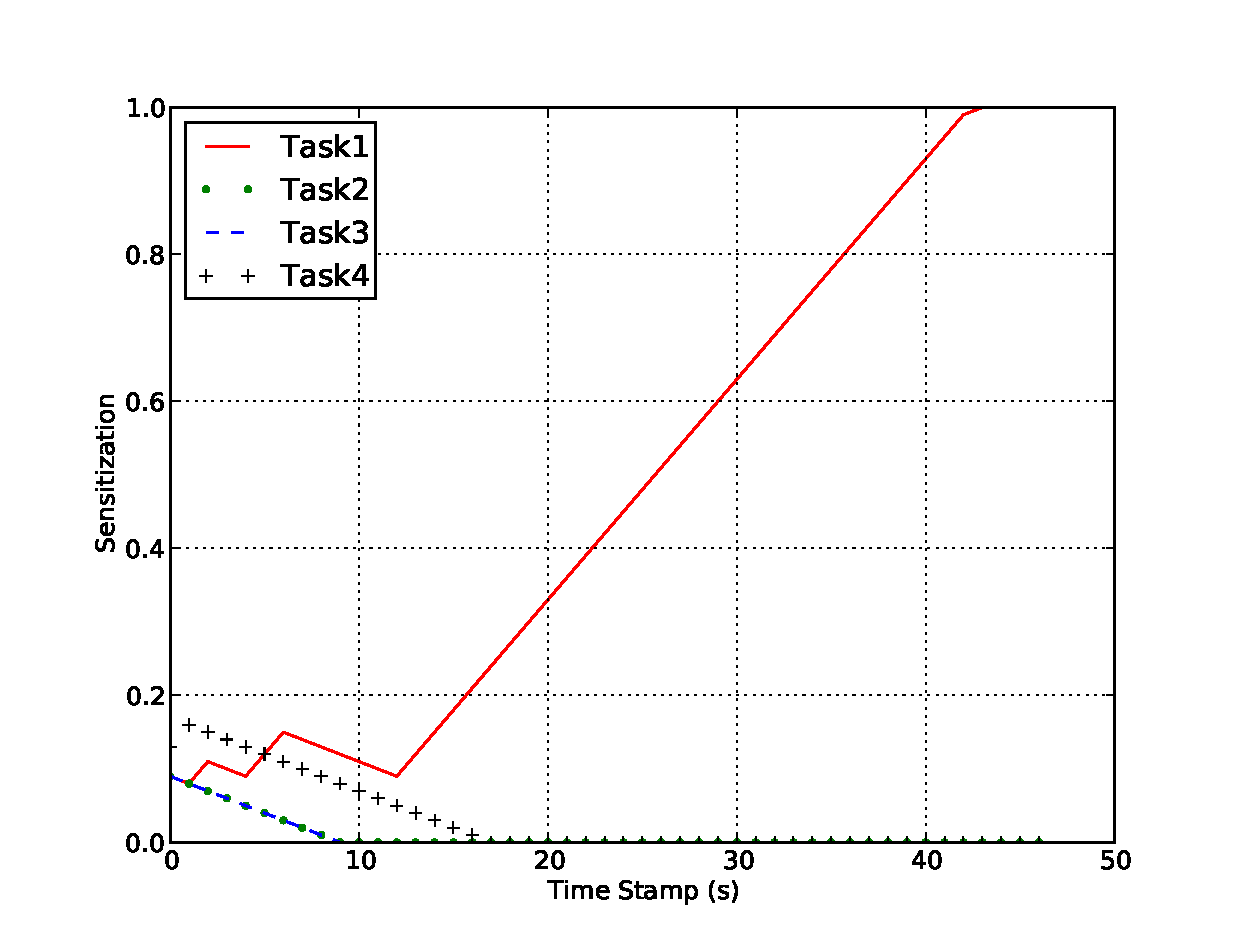
\includegraphics[height=5cm, angle=0]{images/global/PlotRobot9-Sensitizations-2010Feb18-121037.eps}
\caption{\small Task specialization of Robot9 in centralized communication experiments}
\label{fig:single-robot-sensitizations} % Give a unique label
\end{minipage}
\end{figure}
%
%
\section{Conclusion and Future works}
\label{sec:conc}
% Initially robots sensitization to all tasks has been set to 0.1. We set a simple learning rule for sensitization so that if a robot selects a task in Nth step and if the same task has been selected in next (N+1)th step, sensitization of that task (j) for that robot (i) has been increased by a learning coefficient L and at the same time sensitization of other tasks has been decreased by a forgetting coefficient F. This ensures flexibility and concurrency of robots to switch from one task to another.
%
%The global mode experiments have established a base line of self-regulated DoL using broadcast communication strategy.
%As shown in Fig. \ref{fig:2} task urgency varies as robots switch among tasks. %and when 6 robots works in 3 tasks we find a convergence of DoL to near zero.
%
%After some time, when a few working robots have intentionally been removed from the experiment, urgency of some unattended tasks have been increased immediately. When this removed robots return to the experiment urgency of all task again converges to zero. This shows the robustness of AFM for self-regulated DoL. %It relied on decentralized control strategies based on a set of generic rules.
%
%Our future works include iterating above experiments using local and stigmergic communication modes with a larger group of robots (about 40). %The goal is to find out necessary ingredients to reach similar level of self-regulated DoL with varying team sizes.
%\begin{acknowledgements}
%If you'd like to thank anyone, place your comments here
%and remove the percent signs.
%\end{acknowledgements}
% BibTeX users please use one of
%\bibliographystyle{spbasic} % basic style, author-year citations
%\bibliographystyle{spmpsci} % mathematics and physical sciences
%\bibliographystyle{spphys} % APS-like style for physics
%\bibliography{} % name your BibTeX data base
% Non-BibTeX users please use
\begin{thebibliography}{}
%
% and use \bibitem to create references. Consult the Instructions
% for authors for reference list style.
%
\bibitem{Swarm}
% Format for Journal Reference
Erol Sahin and Alan Winfield, Special issue on swarm robotics, Swarm Intelligence, Vol 2, 69-72 (2008)
% Format for books
\bibitem{Elsa}
Elsa Arcaute \textit{et} al., Division of labour in ant colonies in terms of attractive fields, Ecological Complexity, Elsevier (2008)
% etc
\bibitem{SwisTrack}
T. Lochmatter, P. Roduit, C. Cianci, N. Correll, J. Jacot, and A. Martinoli. SwisTrack - A Flexible Open Source Tracking Software for Multi-Agent Systems. In Proceedings of the IEEE/RSJ 2008 International Conference on Intelligent Robots and Systems (IROS 2008), pages 4004-4010. IEEE, 2008.
\bibitem{Epuck}
Mondada, F., Bonani, M., Raemy, X., Pugh, J., Cianci, C., Klaptocz, A., Magnenat, S., Zufferey, J.-C., Floreano, D. and Martinoli, A. (2009) The e-puck, a Robot Designed for Education in Engineering. Proceedings of the 9th Conference on Autonomous Robot Systems and Competitions, 1(1) pp. 59-65.
\bibitem{DBus}
http://www.freedesktop.org/wiki/Software/dbus
\bibitem{Multiprocessing}
http://docs.python.org/library/multiprocessing.html
\bibitem{bustle}
http://willthompson.co.uk/bustle/
\end{thebibliography}
%
\end{document}